\chapter{Desarrollo y experimentación}
\label{ch:desarrollo}

\section{Selección del conjunto de datos}
\label{sec:select_dataset}

En lo que a \textit{malware} se refiere, \textit{BODMAS} \cite{bodmas} es uno de los conjuntos de datos más completos en la actualidad, con la ventaja para este proyecto de ya estar procesado y tener una amplia bibliografía. Otra opción interesante puede ser \textit{VirusShare} \cite{virusshare}, ya que cuenta con más de 99 millones de muestras de \textit{malware} actualizadas pero tiene varios inconvenientes para este proyecto. El primero es que no incluye muestras de \textit{software} no malicioso y el segundo que necesita un procesamiento previo para extraer las características. Todo esto conlleva un aumento considerable para la realización del proyecto. Otra de las opciones estudiadas ha sido \textit{theZoo} \cite{thezoo}. En cuanto a este repositorio hemos podido observar que tiene los mismos inconvenientes que \textit{VirusShare} y no tiene sus ventajas. Por último tenemos \textit{Microsoft Malware Classification} \cite{malware-classification}. En este caso tenemos un conjunto de datos muy amplio con casi medio \textit{terabyte}, pero además de los inconvenientes ya comentados en los anteriores conjuntos, solo incluye \textit{malware} que afecta a equipos \textit{Windows}, lo que limitaría considerablemente el alcance del estudio.

\vspace{1em}

Teniendo en cuenta todo lo comentado hasta ahora sobre los distintos conjuntos de datos considerados, hemos decidido usar \textit{BODMAS}, ya que es el que mejor se adapta a las necesidades del estudio

\newpage
\section{Procesamiento del conjunto de datos}
\label{sec:proc_dataset}

Dadas las limitaciones \textit{hardware} y la cantidad de datos, aproximadamente 135000 patrones y 2400 atributos por cada patrón, es necesario hacer un procesamiento previo del conjunto de datos. Para ello hemos tenido en cuenta varios enfoques. Por un lado, \textit{BODMAS} nos permite hacer una distinción entre clasificación binaria y clasificación multiclase, pero para ello es necesario reordenar los datos, ya que se encuentran distribuidos en varios archivos. Por otro lado, es necesario reducir la cantidad de datos. A continuación veremos los distintos enfoques.

\subsection{Clasificación multiclase}
\label{subsec:multiclass}

El conjunto de datos seleccionado se divide en varios archivos:

\begin{itemize}
	\item \textit{bodmas.npz}: incluye la matriz de patrones de entrada en formato de matriz de \textit{python} y la matriz de salidas deseadas.
	\item \textit{bodmas\_metadata.csv}: la información relevante para nuestro problema es la columna \textit{sha} que contiene la función \textit{hash} de todo el conjunto de datos.
	\item \textit{bodmas\_malware\_category.csv}: contiene la función \textit{hash} del \textit{malware} y la categoría a la que pertenece.
\end{itemize}

Dado que las distintas categorías se encuentran en formato texto, es necesario codificarlas para poder trabajar con ellas. La codificación elegida ha sido la representada en la tabla \ref{tabla:codificacion_malware}.

\vspace{1em}

\begin{table}[th]
	\centering
	\begin{tabular}{ |m{4cm}|c|c| }
		\hline
		\rowcolor{LightCyan}
		Categoría                   & Codificación & Nº de patrones \\
		\hline
		\textit{benign}             & 0            & 77142 \\
		\textit{trojan}             & 1            & 29972 \\
		\textit{worm}               & 2            & 16697 \\
		\textit{backdoor}           & 3            & 7331  \\
		\textit{downloader}         & 4            & 1031  \\
		\textit{informationstealer} & 5            & 448   \\
		\textit{dropper}            & 6            & 715   \\
		\textit{ransomware}         & 7            & 821   \\
		\textit{rootkit}            & 8            & 3     \\
		\textit{cryptominer}        & 9            & 20    \\
		\textit{pua}                & 10           & 29    \\
		\textit{exploit}            & 11           & 12    \\
		\textit{virus}              & 12           & 192   \\
		\textit{p2p-worm}           & 13           & 16    \\
		\textit{trojan-gamethief}   & 14           & 6     \\
		\hline
	\end{tabular}
	\caption{Codificación de las clases \textit{malware}.}
	\label{tabla:codificacion_malware}
\end{table}

Para obtener una nueva matriz de salidas deseadas que incluya los tipos de \textit{malware}, una vez cargados los datos en sus correspondiente variables de \textit{python}, usamos la función \textit{merge} \cite{merge} perteneciente a la clase \textit{pandas.DataFrame} para incluir en \textit{metadata} los datos de \textit{mw\_category['category']} en las entradas donde coincide la columna \textit{sha}.

\vspace{1em}

Antes de codificar necesitamos darle una etiqueta a los datos vacíos, los cuales significan que esa muestra es benigna. Para ello usamos la función \textit{pandas.DataFrame.fillna} \cite{fillna}, que nos permite completar datos vacíos de distintas formas. Para nuestro caso usamos la etiqueta \textit{benign}. También eliminamos las columnas que no vamos a necesitar, dejando solo la categoría a la que pertenece cada muestra.

\vspace{1em}

Ahora podemos codificar los datos usando la función \textit{pandas.DataFrame.map} \cite{map}. Este método aplica una función que acepta y devuelve un valor escalar a cada elemento del DataFrame, lo que permite asignar un valor numérico a cada clase.

\vspace{1em}

El código utilizado para esta tarea se encuentra en el Anexo \ref{sec:codificacion}.

\subsection{Reducción del conjunto de datos}
\label{subsec:red_dataset}

Reducir el número de datos con el que vamos a trabajar tiene el objetivo de principal de disminuir el tiempo que los algoritmos van a necesitar para procesar la información sin perjudicar la integridad de los datos, ya que los resultados del estudio podrían verse afectados y llevar a unas conclusiones erróneas. Esta tarea se puede enfrentar desde dos planteamientos distintos: condensar el número de patrones o el número de características. Ambos planteamientos se han estudiado de forma teórica en esta memoria en las secciones \ref{subsec:balanceo} y \ref{subsec:red_dim} respectivamente. Las técnicas elegidas son \textit{undersampling} por simplicidad y \textit{PCA} porque según el estudio \textit{A Low Complexity ML-Based Methods for Malware Classification} \cite{red_dim_pca} se obtienen unos resultados algo más precisos que con otros métodos.

\vspace{1em}

El código utilizado se encuentra en el anexo \ref{sec:red_dim}. A continuación se explicarán los pasos seguidos.

\subsubsection{Número de patrones}
\label{subsubsec:num_patrones}

Como ya hemos estudiado en la sección \ref{subsubsec:undersampling}, el submuestreo o \textit{undersampling} en inglés, es una técnica para abordar el desbalance de clases en un conjunto de datos, especialmente cuando una de las clases tiene muchos más patrones que la otra. En nuestro caso, el desbalance no es demasiado grande ya que \textit{BODMAS} contiene 57293 muestras \textit{malware} y 77142 muestras benignas.

\vspace{1em}

El método \textit{RandomUnderSampler} \cite{randundersampler} de la librería \textit{Imbalanced learn} nos permite varias formas de actuar, siendo la que nos interesa para este estudio la que nos permite elegir manualmente el número de patrones de cada clase. Hemos elegido una cantidad de 15000 patrones en por clase.

\subsubsection{Número de características}
\label{subsubsec:num_caract}

Este método, también conocido como reducción de la dimensionalidad, consiste en reducir el número de variables de las que consta el problema. Para aplicar el método matemático-estadístico de análisis de componentes principales, \textit{PCA} por sus siglas en inglés, usamos la clase \textit{PCA} \cite{sklearn_pca} perteneciente a \textit{sklearn.decomposition}. Esta clase nos permite entrenar el modelo y transformar el conjunto de datos tanto para el conjunto de entrenamiento como para el de test. Para ello será necesario separar previamente los datos, ya que \textit{BODMAS} no cuenta con esta división.

\subsubsection{Elección final del nuevo conjunto de datos}
\label{subsubsec:eleccion_dataset}

Para poder decidir como será el conjunto de entrenamiento final se han hecho distintos conjuntos de datos sobre los que se probarán algunos algoritmos. Los conjuntos son los siguientes:

\begin{itemize}
	\item Clasificación binaria con \textit{PCA}.
	\item Clasificación binaria con \textit{PCA} y \textit{Undersampling} con 15000 patrones por clase.
	\item Clasificación multiclase con \textit{PCA}.
\end{itemize}

Los resultados obtenidos se reflejan en las tablas \ref{tabla:binary_pca}, \ref{tabla:binary_under} y \ref{tabla:multi_pca} respectivamente.

\begin{table}[th]
	\centering
	\begin{tabular}{ |c|c|c|c|c|c|c|c| }
		\hline
		\rowcolor{LightCyan}
		Clasificador & Tiempo (s) & \multicolumn{3}{c|}{Entrenamiento} & \multicolumn{3}{c|}{Test} \\
		\hline
		\rowcolor{LightCyan}
		&            & Acc & MS & F1 & Acc & MS & F1 \\
		\hline
		\textit{Decission tree} & 0.885 & 1.000 & 1.000 & 1.000 & 0.972 & 0.971 & 1.000 \\
		\textit{Random forest}  & 25.91 & 1.000 & 1.000 & 1.000 & 0.984 & 0.976 & 1.000 \\
		\textit{K-NN}           & 0.095 & 0.973 & 0.970 & 1.000 & 0.963 & 0.963 & 1.000 \\
		\hline
	\end{tabular}
	\caption{Clasificación binaria con \textit{PCA}.}
	\label{tabla:binary_pca}
\end{table}

\begin{table}[th]
	\centering
	\begin{tabular}{ |c|c|c|c|c|c|c|c| }
		\hline
		\rowcolor{LightCyan}
		Clasificador & Tiempo (s) & \multicolumn{3}{c|}{Entrenamiento} & \multicolumn{3}{c|}{Test} \\
		\hline
		\rowcolor{LightCyan}
		&            & Acc & MS & F1 & Acc & MS & F1 \\
		\hline
		\textit{Decission tree} & 0.184 & 1.000 & 1.000 & 1.000 & 0.945 & 0.936 & 1.000 \\
		\textit{Random forest}  & 4.926 & 1.000 & 1.000 & 1.000 & 0.963 & 0.957 & 1.000 \\
		\textit{K-NN}           & 0.016 & 0.954 & 0.948 & 1.000 & 0.938 & 0.931 & 1.000 \\
		\hline
	\end{tabular}
	\caption{Clasificación binaria con \textit{PCA} y \textit{Undersampling}.}
	\label{tabla:binary_under}
\end{table}

\begin{table}[th]
	\centering
	\begin{tabular}{ |c|c|c|c|c|c|c|c| }
		\hline
		\rowcolor{LightCyan}
		Clasificador & Tiempo (s) & \multicolumn{3}{c|}{Entrenamiento} & \multicolumn{3}{c|}{Test} \\
		\hline
		\rowcolor{LightCyan}
		& & Acc & MS & F1 & Acc & MS & F1 \\
		\hline
		\textit{Decission tree} & 1.059 & 0.999 & 0.895 & 0.999 & 0.939 & 0.000 & 0.976 \\
		\textit{Random forest}  & 30.04 & 0.999 & 0.895 & 0.999 & 0.955 & 0.000 & 0.981 \\
		\textit{K-NN}           & 0.088 & 0.951 & 0.000 & 0.981 & 0.936 & 0.000 & 0.975 \\
		\hline
	\end{tabular}
	\caption{Clasificación multiclase con \textit{PCA}}
	\label{tabla:multi_pca}
\end{table}

En cuanto a la clasificación binaria, hemos decidido usar el conjunto de datos en el que se ha aplicado tanto \textit{PCA} como \textit{undersampling}, ya que, aunque los resultados son similares en ambos conjuntos, el tiempo es considerablemente más bajo y dadas las limitaciones del equipo disponible puede ser beneficioso a la hora de probar algoritmos más complejos.

\vspace{1em}

Para la clasificación multiclase hay varios métodos que podemos usar para reducir el tamaño del conjunto de datos, como el \textit{clustering} o variantes del método de \textit{undersampling} ya utilizado en clasificación binaria. A pesar de ello, estos métodos tienen una mayor complejidad de aplicación y la reducción de las dimensiones no es el objeto de este estudio. Por otro lado, esta decisión puede suponer algunos problemas al usar técnicas como \textit{GridSearchCV} o la validación cruzada, ya que incrementan considerablemente el tiempo de entrenamiento.

\vspace{1em}

También en referencia a la clasificación multiclase, podemos ver en la tabla \ref{tabla:multi_pca} que la métrica de mínima sensibilidad es 0 para todos los casos de test. Como ya se ha explicado en esta memoria, mide cómo de bien se clasifica la clase peor clasificada y un valor de 0 indica que alguna de las clases no se ha clasificado bien. Como podemos ver en la matriz de confusión representada en la imagen \ref{fig:confusion}, algunas de las clases con menos patrones tienen dificultades para obtener una buena clasificación debido a la falta de información en el entrenamiento. Algunos clasificadores tienen la opción de asignar un peso a los patrones de cada clase inversamente proporcional al número de patrones de la clase, de manera que todas las clases tengan el mismo peso en el entrenamiento, pero no se consiguen mejores resultados. 

\begin{figure}[H]
	\centering
	% include first image
	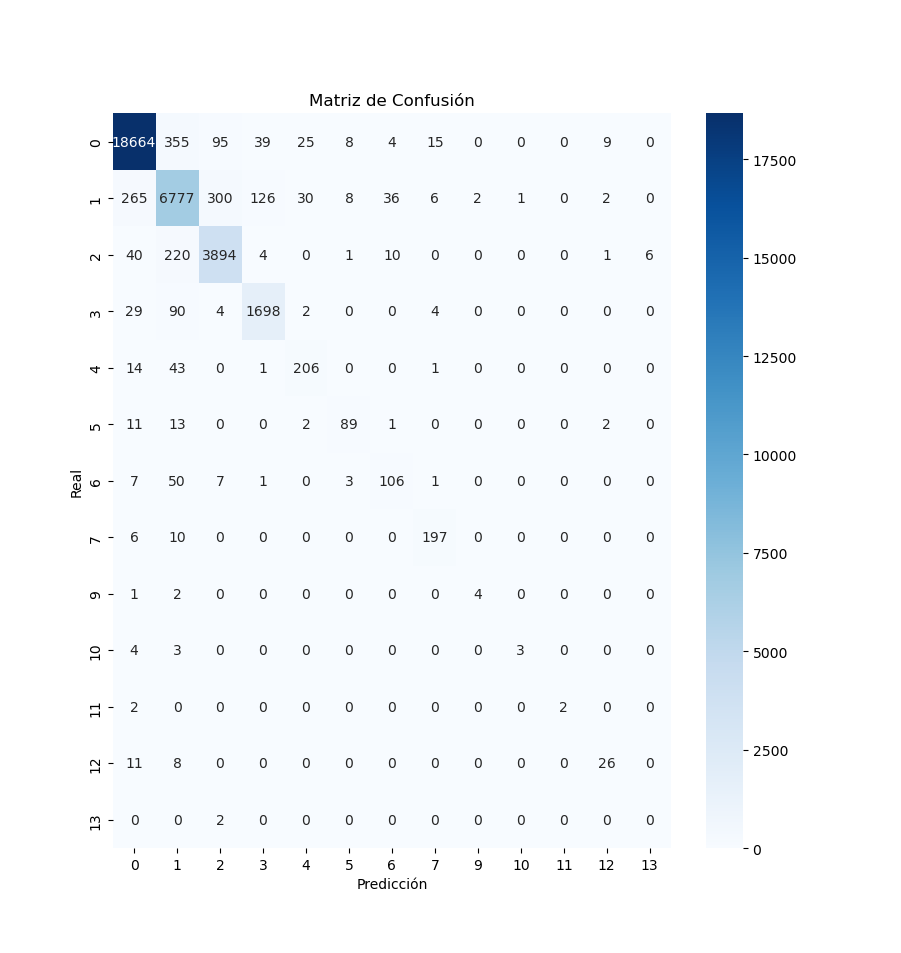
\includegraphics[width=1.2\linewidth]{Imagenes/confusion_multiclase}
	\caption[Titulo de la figura para el índice de figuras. En este no se deben poner referencias a citas]{Título de la figura para el texto}
	\label{fig:confusion}
\end{figure}

Según el estudio \textit{Malware Behavior Analysis: Learning and Understanding Current Malware Threats} \cite{mba}, algunos de los tipos de \textit{malware} que tenemos con menos patrones, se pueden agrupar en algunas de las clases más representadas de nuestro conjunto de datos. En este estudio se comenta que \textit{p2p-worm} añade un comportamiento específico al comportamiento de un gusano, generando problemas de red y de pérdida de datos. Algo similar pasa con \textit{Gamethief trojan}. De esta forma podemos agrupar estos patrones a sus respectivas clases similares sin perder efectividad a la hora de clasificar y además eliminar así dos de las clases que nos pueden dar problemas por falta de información.

\vspace{1em}

Por otro lado, se han planteado dos formas de solucionar este problema, aunque ambas presentan inconvenientes:

\begin{itemize}
	\item Eliminar las clases menos representadas. Tiene el riesgo de no reconocer un nuevo patrón si es de un tipo distinto de \textit{malware}.
	\item Agruparlas en una nueva clase que represente varios tipos de \textit{malware}. En este caso estamos suponiendo que los patrones agrupados tienen unas características similares.
\end{itemize}

\vspace{1em}

Finalmente hemos decidido agrupar las clases con menos de 30 patrones en una nueva categoría \textit{otros}. Por número de patrones sería recomendable agrupar también la clase \textit{virus}, pero podría tener demasiado peso en la categoría otros y hemos considerado que es lo suficientemente relevante como para estudiarla por separado. En la tabla \ref{tabla:multi_new} podemos ver que, aunque mejoramos la mínima sensibilidad, no se producen unas mejoras significativas en la precisión de clasificación pero dada la alta precisión presentada por los modelos y la mejora en la mínima sensibilidad puede considerarse una buena actualización. Podemos ver la nueva codificación en la tabla \ref{tabla:nueva_codificacion_malware}

\begin{table}[th]
	\centering
	\begin{tabular}{ |m{4cm}|c|c| }
		\hline
		\rowcolor{LightCyan}
		Categoría                   & Codificación & Nº de patrones \\
		\hline
		\textit{benign}             & 0            & 77142 \\
		\textit{trojan}             & 1            & 29978 \\
		\textit{worm}               & 2            & 16713 \\
		\textit{backdoor}           & 3            & 7331  \\
		\textit{downloader}         & 4            & 1031  \\
		\textit{informationstealer} & 5            & 448   \\
		\textit{dropper}            & 6            & 715   \\
		\textit{ransomware}         & 7            & 821   \\
		\textit{virus}              & 8            & 192   \\
		\textit{otros}              & 9            & 64    \\
		\hline
	\end{tabular}
	\caption{Nueva codificación de las clases \textit{malware}.}
	\label{tabla:nueva_codificacion_malware}
\end{table}

\begin{table}[th]
	\centering
	\begin{tabular}{ |c|c|c|c|c|c|c|c| }
		\hline
		\rowcolor{LightCyan}
		Clasificador & Tiempo (s) & \multicolumn{3}{c|}{Entrenamiento} & \multicolumn{3}{c|}{Test} \\
		\hline
		\rowcolor{LightCyan}
		&            & Acc & MS & F1 & Acc & MS & F1 \\
		\hline
		\textit{Decission tree} & 1.220  & 0.998 & 0.992 & 0.998 & 0.938 & 0.670 & 0.975 \\
		\textit{Random forest}  & 31.201 & 0.998 & 0.993 & 0.998 & 0.953 & 0.670 & 0.980 \\
		\textit{K-NN}           & 0.083  & 0.951 & 0.431 & 0.980 & 0.936 & 0.333 & 0.974 \\
		\hline
	\end{tabular}
	\caption{Clasificación multiclase con la nueva codificación.}
	\label{tabla:multi_new}
\end{table}


\vspace{1em}

Por último, se han considerado otras opciones para mejorar la clasificación de las clases minoritarias, pero podrían exceder la complejidad de este proyecto:

\begin{itemize}
	\item Utilizar métodos de sobremuestreo, ya mencionados en la sección \ref{subsubsec:oversampling}, que consisten en aumentar la cantidad de patrones de estas clases de forma sintética.
	\item Utilizar métodos jerárquicos que primero clasifiquen usando la categoría \textit{otros}, para después dividirla en sus diferentes clases y entrenar un modelo específico.
\end{itemize}

\section{Experimentación}
\label{sec:exp}

\subsection{Clasificación binaria}
\label{sec:clas_binaria}

\subsubsection{Árboles de decisión}
\label{sec:dec_tree}

\begin{table}[th]
	\centering
	\begin{tabular}{ |c|c|c|c|c|c|c| }
		\hline
		\rowcolor{LightCyan}
		 & \multicolumn{3}{c|}{Entrenamiento} & \multicolumn{3}{c|}{Test} \\
		\hline
		\rowcolor{LightCyan}
		 Estado aleatorio & Acc & MS & F1 & Acc & MS & F1 \\
		\hline
		0 & 1.000 & 1.000 & 1.000 & 0.951 & 0.942 & 1.000 \\
		1 & 1.000 & 1.000 & 1.000 & 0.944 & 0.935 & 1.000 \\
		2 & 1.000 & 1.000 & 1.000 & 0.942 & 0.935 & 1.000 \\
		3 & 1.000 & 1.000 & 1.000 & 0.948 & 0.938 & 1.000 \\
		4 & 1.000 & 1.000 & 1.000 & 0.953 & 0.946 & 1.000 \\
		5 & 0.998 & 0.997 & 1.000 & 0.947 & 0.936 & 1.000 \\
		6 & 0.998 & 0.997 & 1.000 & 0.947 & 0.941 & 1.000 \\
		7 & 1.000 & 1.000 & 1.000 & 0.949 & 0.946 & 1.000 \\
		8 & 0.999 & 0.998 & 1.000 & 0.948 & 0.937 & 1.000 \\
		9 & 1.000 & 1.000 & 1.000 & 0.950 & 0.940 & 1.000 \\
		Mean & 0.999 & 0.999 & 1.000 & 0.948 & 0.940 & 1.000 \\
		STD & 0.001 & 0.001 & 0.000 & 0.003 & 0.004 & 0.000 \\
		\hline
	\end{tabular}
	\caption{caption}
	\label{label}
\end{table}

